\documentclass[10pt,oneside,final]{amsart}
\usepackage[letterpaper]{geometry}
\usepackage[lmodern,cat]{trinh-m-q_14_10}
\usepackage{tikz-cd}

\begin{document}

%	Title block

\title{The Functor of Points}
%		\dedicatory{}
\date{29 January 2014. Last rev.~\today}
%		\subjclass[2010]{}
%		\keywords{}
%		\thanks{Advised by Shou-Wu Zhang}

%	Author block(s)

\author{Minh-Tam Trinh}
\address{Department of Mathematics, Princeton University, Princeton, NJ 08544}
\email{\href{mailto:mqtrinh@gmail.com}{mqtrinh@gmail.com}}

\maketitle

\thispagestyle{empty}

%--------------------------------------------------------------------------

\textbf{Spoiler Alert:}
We solve some exercises in \cite{EH}.

\section{The Yoneda Lemma}

Let $\sf{C}$ be a locally small category.
If $X \in \sf{C}$, then the \emph{(covariant) hom functor} of $X$ is the functor $h^X : \sf{C} \to \Set$ that sends $Y \mapsto \Hom(X, Y)$, and sends $g : Y_1 \to Y_2$ to the operation of postcomposition with $g$.

\begin{lem}[Yoneda]\label{00}
Let $\cal{F} : \sf{C} \to \Set$ be arbitrary, and let $X \in \sf{C}$.
Then the map
\begin{align}
\Phi \mapsto \Phi_X(\id_X)
\end{align}
is a natural bijection $\Hom(h^X, \cal{F}) \to \cal{F}(X)$.
\end{lem}

\begin{proof}
For all $Y \in \sf{C}$ and $f \in \Hom(X, Y)$, there is a commutative diagram:
\begin{equation}
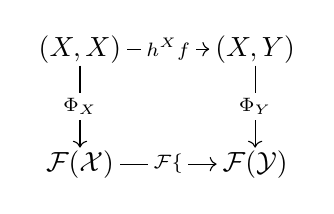
\begin{tikzpicture}[baseline=(current  bounding  box.center)]
\tikzstyle{every node}=[fill=white,  inner sep=2pt]
\matrix (m)
[	matrix of math nodes,
	row sep 		=	3em,
	column sep 	=	3em,
	text height	=	1.5ex,
	text depth	=	0.25ex
]
{ 		\Hom(X, X) 			&\Hom(X, Y)\\
		\cal{F}(X)				&\cal{F}(Y)		\\
};
\path[->, font=\scriptsize]
(m-1-1) edge node 	{$h^X f$}					(m-1-2)
(m-1-1) edge node	{$\Phi_X$}					(m-2-1)
(m-1-2) edge node	{$\Phi_Y$}					(m-2-2)
(m-2-1) edge node 	{$\cal{F} f$}					(m-2-2);
\end{tikzpicture}
\end{equation}
In particular, $(\cal{F} f)(\Phi_X(\id_X)) = \Phi_Y(f)$, which shows that $\Phi$ is uniquely determined by $a = \Phi_X(\id_X)$ and any choice of $a \in \cal{F}(X)$ is possible.
\end{proof}

In the notation of \ref{00}, let $a \in \cal{F}(X)$.
We say that the pair $(X, a)$ \emph{represents} $\cal{F}$ iff the natural transformation $h^X \to \cal{F}$ corresponding to $a$ is an isomorphism.
If $\cal{F}$ is representable, then \ref{00} implies the representing object is unique up to unique isomorphism.

\begin{cor}\label{01}
The functor $X \mapsto h^X$ is a full and faithful embedding $\sf{C} \to \Fun(\sf{C}, \Set)$.
\end{cor}

Recall that a \emph{presheaf} on $\sf{C}$ is another name for a contravariant functor $\sf{C} \to \Set$.
We write $\PSh(\sf{C}) = \Fun(\sf{C}, \Set^\op)$ for the category of presheaves on $\sf{C}$.
The \emph{contravariant hom functor} of $X$ is the presheaf $h_X : \sf{C} \to \Set$ that sends $Y \mapsto \Hom(Y, X)$, and sends $g : Y_1 \to Y_2$ to precomposition with $g$.
Thus, the dual of \ref{01} says that the map $X \mapsto h_X$ is a full and faithful embedding $\sf{C} \to \PSh(\sf{C})$.
The maps $X \mapsto h^X$ and $X \mapsto h_X$ are called the \emph{Yoneda embeddings}.

The utility of the Yoneda embedding is this:
First, it lets us generalize properties of objects of $\sf{C}$ in a natural way to properties of functors or presheaves on $\sf{C}$.
Second, the category of functors from $\sf{C}$ to $\Set$ or $\Set^\op$ is often more well-behaved than $\sf{C}$ itself: 
We may be able to perform constructions in the larger category that we could not do in $\sf{C}$.
For example, $\sf{C}$ may not contain fiber products, whereas the new category does.

\section{$R$-Functors}

Fix a ring $R$.
Take $\sf{C} = \Sch/R$, the category of schemes over $\Spec R$, so that if $R = \Z$, then $\Sch/R = \Sch$.
In this setting, we say that $h_X$ is the \emph{functor of points of $X$}, and that the elements of $h_X(Y)$ are the \emph{$Y$-valued points of $X$}.
If $A$ is a ring, then we abbreviate $h_X(A) = h_X(\Spec A)$.

We can sharpen \ref{01} slightly:
It turns out that the functor of points of an $R$-scheme is completely determined by how it behaves on the spectra of $R$-algebras.
Let $\Ring(R)$ be the category of $R$-algebras, and for all $X \in \Sch/R$, let
\begin{align}
h_X^\ast = h_X \circ \Spec : \Ring(R) \to \Set
\end{align}
be the (covariant!) functor that sends $A \mapsto h_X(A) = \Hom_{\Sch/R}(\Spec A, X)$.

\begin{cor}\label{02}
If $R$ is a ring, then the functor  $X \mapsto h_X^\ast$ is a full and faithful embedding $\Sch/R \to \Fun(\Ring(R), \Set)$.
\end{cor}

\begin{proof}
Let $X, Y \in \Sch/R$.
We must show that every natural transformation $\Phi : h_Y^\ast \to h_X^\ast$ comes from a unique $\Sch/R$ morphism $Y \to X$.
Take an affine open cover $\{V_j\}$ of $Y$, and let $\iota_j : V_j \to Y$ be the inclusion map.
Then $\Phi(\iota_j)$ is a $\Sch/R$ morphism $V_j \to X$, and by compatibility, the family $\{\Phi(\iota_j)\}$ determines a unique $\Sch/R$ morphism on $Y$.
\end{proof}
 
We will now generalize our topological notions about $R$-schemes to notions about functors $\Ring(R) \to \Set$, which we call \emph{$R$-functors}. 
First, check that if $\Phi_1 : \cal{F}_1 \to \cal{G}$ and $\Phi_2 : \cal{F}_2 \to \cal{G}$ are $R$-functor morphisms, then the fiber product $\cal{F}_1 \times_\cal{G} \cal{F}_2$ in the category $\Fun(\Ring(R), \Set)$ is realized by the functor that sends
\begin{align}\label{EQ:03}
A \mapsto \{(a_1, a_2) \in \cal{F}_1(A) \times \cal{F}_2(A) : \Phi_{1, A}(a_1) = \Phi_{2, A}(a_2)\}.
\end{align}
It follows that $X \mapsto h^\ast_X$ preserves fiber products:
For all $X, Y_1, Y_2 \in \Sch/R$,
\begin{align}\label{EQ:00}
h_{Y_1 \times_X Y_2}^\ast = h_{Y_1}^\ast \times_{h_X^\ast} h_{Y_2}^\ast.
\end{align}
Let $\cal{F}$ be an $R$-subfunctor of $\cal{G}$, meaning there is a morphism $\cal{F} \to \cal{G}$ such that $\cal{F}(A) \to \cal{G}(A)$ is injective for all $A$.
We say that $\cal{F}$ is \emph{open (resp., closed) in $\cal{G}$} iff, for all $R$-schemes $X$ and $R$-functor morphisms $h_X^\ast \to \cal{G}$, the base change $\cal{F} \times_\cal{G} h_X^\ast$ is isomorphic to $h_Y^\ast$ for some open (resp., closed) subscheme $Y$ of $X$.


\begin{lem}\label{03}
Let $R$ be a ring.
If $X \in \Sch/R$, then the open (resp., closed) $R$-subfunctors of $h_X^\ast$ are the functors of the form $h_Y^\ast$ for some open (resp., closed) subscheme $Y$ of $X$.
\end{lem}

\begin{proof}
By (\ref{EQ:00}) and the compatibility of open (resp., closed) immersions with respect to base change, every functor of the form $h_Y^\ast$ with $Y$ an open (resp., closed) subscheme of $X$ is an open (resp., closed) subfunctor of $h_X^\ast$.
The reverse inclusion follows from considering the trivial base change to $h_X^\ast$ itself.
\end{proof}

\begin{prop}
Let $R$ be a ring, and let $A \in \Ring(R)$.
\begin{enumerate}
\item 	The open $R$-subfunctors of $h_{\Spec A}^\ast$ are the functors of the form
\begin{align}\label{EQ:01}
B \mapsto \{f \in h_{\Spec A}^\ast(B) : f_{\Spec A}^\#(\fr{a})B = B\}
\end{align}
for some $\fr{a} \normal A$.
\item 	The closed $R$-subfunctors of $h_{\Spec A}^\ast$ are the functors of the form
\begin{align}\label{EQ:02}
B \mapsto \{f \in h_{\Spec A}^\ast(B) : f_{\Spec A}^\#(\fr{a})B \subeq \nil B\}
\end{align}
for some $\fr{a} \normal A$.
\end{enumerate}
\end{prop}

\begin{proof}\mbox{}
\begin{enumerate}
\item 	The open subsets of $\Spec A$ take the form $D(\fr{a}) = \Spec A \setminus V(\fr{a})$ for some $\fr{a} \normal A$.
			By \ref{03}, it suffices to prove that if $\phi : A \to B$ is a $\Ring(R)$ morphism, then $\phi(\fr{a})B = B$ if and only if $f = \Spec(\phi) : \Spec B \to \Spec A$ has image in $D(\fr{a})$.
			The latter occurs if and only if $\fr{a} \not\subeq \phi^{-1}(\fr{q})$ for all $\fr{q} \in \Spec B$, meaning there exists $b \in \phi(\fr{a})\setminus \fr{q}$ for all such $\fr{q}$.
			In particular, this happens if and only if $\phi(\fr{a})$ contains a unit, as we see from considering maximal $\fr{q}$; this means $\phi(\fr{a})B$ contains $1$.
\item 	Let $\fr{a} \normal A$.
			By \ref{03}, it suffices to prove that if $\phi : A \to B$ is a $\Ring(R)$ morphism, then $\phi(\fr{a})B\subeq \nil B$ if and only if $f = \Spec(\phi) : \Spec B \to \Spec A$ has image in $V(\fr{a})$.
			The latter occurs if and only if $\fr{a} \subeq \phi^{-1}(\fr{q})$ for all $\fr{q} \in \Spec B$, meaning $\phi(\fr{a}) \subeq \bigcap_{\fr{q} \in \Spec B} = \nil B$.
\end{enumerate}
\end{proof}

We write $U_\fr{a}$ and $Z_\fr{a}$ for the functors defined in (\ref{EQ:01}) and (\ref{EQ:02}), respectively.
Note that in general, $U_\fr{a}(B) \cup Z_\fr{a}(B) \neq h_{\Spec A}^\ast(B)$; however, equality holds if, for example, $B$ is a DVR or a field.

Suppose $\{\cal{U}_i\}$ is a family of open $R$-subfunctors of $\cal{F}$.
We say that $\{\cal{U}_i\}$ is an \emph{open cover of $\cal{F}$} iff, for all $R$-schemes $X$ and $R$-functor morphisms $h_X^\ast \to \cal{F}$ such that $\cal{U}_i \times_\cal{F} h_X^\ast = h_{U_i}^\ast$, the family $\{U_i\}$ is an open cover of $X$.

\begin{ex}
It is false that if $\{\cal{U}_i\}$ is an open cover of $\cal{F}$, then $\cal{F}(A) = \bigcup_i \{\cal{U}_i(A)\}$ for all $A \in \Ring(R)$.
For example, take $R = \Z$.
If $p, q$ are distinct primes, then 
\begin{align}
\{h_{\Spec \Z[1/p]}^\ast, h_{\Spec \Z[1/q]}^\ast\}
\end{align}
is a cover of $h_{\Spec \Z}^\ast$, but $h_{\Spec \Z}^\ast(\Spec \Z) = \{\id_{\Spec \Z}\}$, whereas 
\begin{align}
h_{\Spec \Z[1/p]}^\ast(\Spec \Z) = h_{\Spec \Z[1/q]}^\ast(\Spec \Z) = \emptyset
\end{align}
\cite[p.~255]{EH}.
\end{ex}

\begin{prop}
Let $\{\cal{U}_i\}$ be a family of open $R$-subfunctors of $\cal{F}$.
Then $\{\cal{U}_i\}$ is an open cover of $\cal{F}$ if and only if $\cal{F}(\F) = \bigcup_i \cal{U}_i(\F)$ for all fields $\F \in \Ring(R)$.
\end{prop}

\begin{proof}
To prove the ``only if'' direction:
Suppose $\{\cal{U}_i\}$ is an open cover of $\cal{F}$.
Let $\F \in \Ring(R)$ be a field.
We have $h_{\Spec \F}^\ast = h^\F$, so by the Yoneda Lemma, it suffices to show $\Hom(h_{\Spec \F}^\ast, \cal{F}) \subeq \bigcup_i \Hom(h_{\Spec \F}^\ast, \cal{U}_i)$.

Fix $\Phi \in \Hom(h_{\Spec \F}^\ast, \cal{F})$.
For all $i$, the base change $\cal{U}_i \times_\cal{F} h_{\Spec \F}^\ast$ with respect to $\Phi$ is either $h_{\emptyset}^\ast$ or $h_{\Spec \F}^\ast$, which forces $\cal{U}_j \times_\cal{F} h_{\Spec \F}^\ast = h_{\Spec \F}^\ast$ for some $j$.
Explicitly, this means $\Phi$ defines a morphism $h_{\Spec \F}^\ast \to \cal{U}_j$, as needed.

To prove the ``if'' direction:
Suppose $\cal{F}(\F) = \bigcup_i \cal{U}_i(\cal{F})$ for all fields $\F$.
Let $X \in \Sch/R$.
By the transitivity of base change, we can assume $X = \Spec A$ for some $A \in \Ring(R)$.
If $\fr{p} \in X$, then we write $k(\fr{p}) = A_\fr{p}/\fr{p} A_\fr{p}$.
For all $\fr{p}$, there exists $i$ such that $\cal{U}_i \times_\cal{F} h_{k(\fr{p})}^\ast = h_{k(\fr{p})}^\ast$ by the Yoneda Lemma.
Therefore, writing $h_{U_i}^\ast = \cal{U}_i \times_\cal{F} h_X^\ast$,
\begin{align}
h_{k(\fr{p})}^\ast
&=		\cal{U}_i \times_\cal{F} h_{k(\fr{p})}^\ast \times_{h_X^\ast} h_X^\ast
			\\
&=		h_{U_i}^\ast \times_{h_X^\ast} h_{k(\fr{p})}^\ast
			\nn
&=		h^\ast_{U_i \times_X k(\fr{p})}.
			\n
\end{align}
This can happen only if $\fr{p} \in U_i$.
Therefore, $\{U_i\}$ is an open cover of $X$.
\end{proof}

%--------------------------------------------------------------------------

\begin{thebibliography}{.....  ..}
\bibitem[EH]{EH}
	D.\ Eisenbud \& J.\ Harris.
	\emph{The Geometry of Schemes}.
	Springer-Verlag
	(2000).
\end{thebibliography}

\end{document}
